\documentclass[11pt, letterpaper]{article}
\usepackage[utf8]{inputenc}

\makeatletter
\newcommand{\@BIBLABEL}{\@emptybiblabel}
\newcommand{\@emptybiblabel}[1]{}
\newcommand*{\permcomb}[4][0mu]{{{}^{#3}\mkern#1#2_{#4}}}
\newcommand{\perm}[1][-3mu]{\permcomb[#1]{P}}
\makeatother
\usepackage[hidelinks]{hyperref}
\usepackage{comment}
\usepackage{enumitem}
\usepackage{fullpage}
\usepackage[english]{babel}
\usepackage{graphicx}
\usepackage[colorinlistoftodos]{todonotes}
\usepackage[linesnumbered]{algorithm2e}
\usepackage{tabularx}
\usepackage{url}
\usepackage{hyperref}
\hypersetup{colorlinks=true}
\usepackage[margin=0.7in]{geometry}    % For reducing margin
\usepackage[english]{babel}
\usepackage{mathtools}
\usepackage{booktabs}
\usepackage{physics}
\usepackage{amsmath,amssymb,amsthm}
\usepackage{fullpage}
\usepackage{enumitem}
\usepackage{tcolorbox}
\usepackage{comment}
\usepackage{framed}

\newcommand{\wx}[1]{\textcolor{magenta}{\bf\small [#1 --WX]}}

\begin{document}

\title{CS 7650: Natural Language Processing (Spring 2024) \\ Problem Set 2}
\author{Instructor: Wei Xu \\ TAs: Andrew Li, Anton Lavrouk, Marcus Ma
\\Piazza: \url{https://piazza.com/gatech/spring2024/cs7650a}
\\Gradescope: \url{https://www.gradescope.com/courses/697909}}
\date{Due: Monday, March 11, 11:59 PM ET}
\maketitle

\section{Hidden Markov Models and the Viterbi Algorithm}
    We have a toy language with 2 words - “cool” and “shade”. We want to tag the parts of speech in a test corpus in this toy language. There are only 2 parts of speech — NN (noun) and VB (verb) in this language. We have a corpus of text in which we the following distribution of the 2 words:
    
    \begin{table}[h!]
    \centering
    \small
    \begin{tabular}{|l | c | c |}
    \hline & NN & VB\\
    \hline
    cool & 15 & 6 \\
    shade & 5 & 9\\
    \hline
    \end{tabular}
    \end{table}
    Assume that we have an HMM model with the following transition probabilities (* is a special start of the sentence symbol).
    
    \begin{figure}[h]
    \centering
    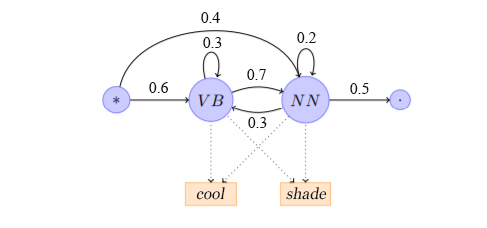
\includegraphics{images/HMM.jpg}
    \caption{HMM model for POS tagging in our toy language.}
    \end{figure}

\begin{enumerate}[label=(\alph*)]
\item (\textbf{2 pts}) Compute the emission probabilities for each word given each POS tag.\\

\item (\textbf{3 pts}) Draw the Viterbi trellis for the sequence “cool shade.” (Do include the period!). Highlight the most likely sequence. \href{https://web.stanford.edu/~jurafsky/slp3/A.pdf#page=8}{\color{blue}{Here}} is an  example of Viterbi trellis.

\end{enumerate}

\newpage

\section{LSTMs vs Transformers}

Both LSTMs and Transformers can be thought of as a transformation from a sequence of input vectors $\textbf{x}_1, \textbf{x}_2, \dots \textbf{x}_n \in \mathbb{R}^d$ to a sequence of outputs $\textbf{h}_1, \textbf{h}_2, \dots, \textbf{h}_n \in \mathbb{R}^d$ (for simplicity, we assume their dimensions are the same). Let's compare the running time of an LSTM layer and a (single-head) self-attention layer in a Transformer:

\begin{itemize}
    \item LSTM:

    $$\begin{aligned}
        \mathbf{f}_i &= \sigma(\mathbf{W}^{(f)}\mathbf{h}_{i-1} + \mathbf{U}^{(f)}\mathbf{x}_i)\\
        \mathbf{i}_i &= \sigma(\mathbf{W}^{(i)}\mathbf{h}_{i-1} + \mathbf{U}^{(i)}\mathbf{x}_i)\\
        \mathbf{g}_i &= \tanh(\mathbf{W}^{(g)}\mathbf{h}_{i-1} + \mathbf{U}^{(g)}\mathbf{x}_i)\\
        \mathbf{o}_i &= \sigma(\mathbf{W}^{(o)}\mathbf{h}_{i-1} + \mathbf{U}^{(o)}\mathbf{x}_i)\\
        \mathbf{c}_i &= \mathbf{f}_i \odot \mathbf{c}_{i-1} + \mathbf{i}_i \odot \mathbf{g}_i\\
        \mathbf{h}_i &= \mathbf{o}_i \cdot \tanh(\mathbf{c}_i)\\
    \end{aligned}$$

    where $\mathbf{W}^{(f)},\mathbf{W}^{(i)},\mathbf{W}^{(g)},\mathbf{W}^{(o)},\mathbf{U}^{(f)},\mathbf{U}^{(i)},\mathbf{U}^{(g)},\mathbf{U}^{(o)}\in\mathbb{R}^{d\times d}$ (bias terms not shown).

    \item Self-attention:
        $$\begin{aligned}
            \mathbf{q}_i &= \mathbf{W}^{(q)}\mathbf{x}_i\\
            \mathbf{k}_i &= \mathbf{W}^{(k)}\mathbf{x}_i\\
            \mathbf{v}_i &= \mathbf{W}^{(v)}\mathbf{x}_i\\
            \mathbf{h}_i &= \mathbf{W}^{(o)} \sum_{j=1}^n \left(\frac{\exp(\mathbf{q}_i\cdot \mathbf{k}_j / \sqrt{d})}{\sum_{j'=1}^n\exp(\mathbf{q}_i\cdot \mathbf{k}_{j'} / \sqrt{d})} \mathbf{v}_j\right) \\
        \end{aligned}$$

        where $\mathbf{W}^{(q)},\mathbf{W}^{(k)},\mathbf{W}^{(v)},\mathbf{W}^{(o)},\in\mathbb{R}^{d\times d}$ (bias terms not shown).
\end{itemize}

\begin{enumerate}
    \item \textbf{(2 points)} Compare the running time of the forward pass of these two models in big $\mathcal{O}$ notations in terms of $n$ and $d$. 
    
    \item \textbf{(3 point)} Suppose that we want to run these two models on long sequences $n \gg d$ (e.g. $d = 512, n = 4096$), which model runs faster in theory? In practice, which model is easier to parallelize? Which model is better at capturing long-term dependencies? Provide a brief reason for each answer.
\end{enumerate}
    

\newpage

\section{Byte-Pair Encoding}

\begin{enumerate}

    \item \textbf{(2 points)} You are given a training corpus of the following strings: \{\colorbox{blue!10}{\textbf{crazy\_}}, \colorbox{blue!10}{\textbf{hazy\_}}, \colorbox{blue!10}{\textbf{day\_}}\}.  Here, \colorbox{blue!10}{\textbf{\textunderscore}} represents the end of a word.

     Apply byte-pair encoding algorithm for \textbf{three} iterations to learn the subword units for this corpus. For each iteration, show the selected merge-operation and its corresponding score. Also, report the initial vocabulary and the final vocabulary at the end. If there are any ties, you can use any option.
    
    \item \textbf{(1 point)} Tokenize the word \colorbox{blue!10}{\textbf{lazy}} using the merging operations from part (i). You are expected to append  \colorbox{blue!10}{\textbf{\textunderscore}} to the word before tokenizing it. Replace any out of vocabulary sub-words or characters with an \colorbox{blue!10}{\textbf{$<$unk$>$}} token.


     \item \textbf{(1 point)} Now consider the following variant of the byte-pair encoding algorithm. Instead of computing counts to choose the best bigram, the variant computes a score for each pair of tokens $x$ and $y$ as follows:

     \begin{equation*}
        score(x, y) = \frac{\textit{frequency of bigram }\textit{xy}}{\textit{frequency of }\textit{x}\;\;\times\;\;\textit{frequency of }\textit{y}}  
     \end{equation*}

     Apply the new variant of byte-pair encoding on the given sentence for \textbf{three} iterations. The new training corpus is \{\colorbox{blue!10}{\textbf{crazy\_}}, \colorbox{blue!10}{\textbf{hazy\_}}, \colorbox{blue!10}{\textbf{phase\_}}\}. For each iteration, show the selected merge-operation and its corresponding score. Also, report the initial and the final vocabularies. In case of any ties, feel free to choose any option.

   \item \textbf{(1 point)} Tokenize the word \colorbox{blue!10}{\textbf{crayon}} using the new set of merging operations from part (3). Once again, you are expected to append  \colorbox{blue!10}{\textbf{\textunderscore}} to the word before tokenizing it. Replace any out of vocabulary sub-words or characters with an \colorbox{blue!10}{\textbf{$<$unk$>$}} token.

\end{enumerate}

\newpage

\section{Beam Search Decoding}
Consider the following bigram language model. The bigram probabilities are given in table \ref{tab:bigram_prob}. Each probability is of the form $P(x_i|x_{i-1})$, where $x_i$ corresponds to $i^{th}$ word in a post / word sequence. Here, $\langle s \rangle$ denotes the start of a sentence.

\begin{table}[h!]
    \centering
    \begin{tabular}{|l|c|l|c|}
    \toprule
        Bigram & Prob. & Bigram & Prob.\\
        \hline
        P(, $|$ know) & 0.3 & P(important $|$ the) & 0.2 \\
        P(the $|$ know) & 0.7 & P(response $|$ correct) & 0.4 \\
        P(I $|$ ,) & 0.6 & P(answer $|$ correct) & 0.35  \\
        P(it $|$ ,) & 0.4 & P(problems $|$ correct) & 0.25  \\
        P(will $|$ I) & 0.2 & P(response $|$ important) & 0.1 \\
        P(know $|$ I) & 0.8 & P(answer $|$ important) & 0.9\\
        P(was $|$ it) & 1.0 & P(answer $|$ exact) & 1.0 \\
        P(correct $|$ the) & 0.3 &  P(exact $|$ the) & 0.5 \\
    \bottomrule
    \end{tabular}
    \caption{Bigram Language Model probabilities for Beam Search.}
    \label{tab:bigram_prob}
\end{table}

\begin{enumerate}
    \item (\textbf{3 pts}) Given a prefix string ``$\langle s\rangle\;I\;know$'', what are the next $3$ possible tokens. Run beam search with width $k=2$ and generate the next $3$ tokens. 
    
    Assume $P(\langle s  \rangle\;I\;know) = 1$. Make sure you show the probabilities for each step. Also, show the word sequences in the beam at the end of each step.
    
    \item Lets introduce some randomness into the standard beam search method used in question $3.1$. At the end of each step, we randomly choose one of the top-k beam candidates and discard the rest. In other words, only the randomly chosen top-k candidate is expanded in the next step instead of all the top-k candidates. Figure \ref{fig:top_k} illustrates this sampling approach.
    
    \begin{figure}[h!]
    \centering
    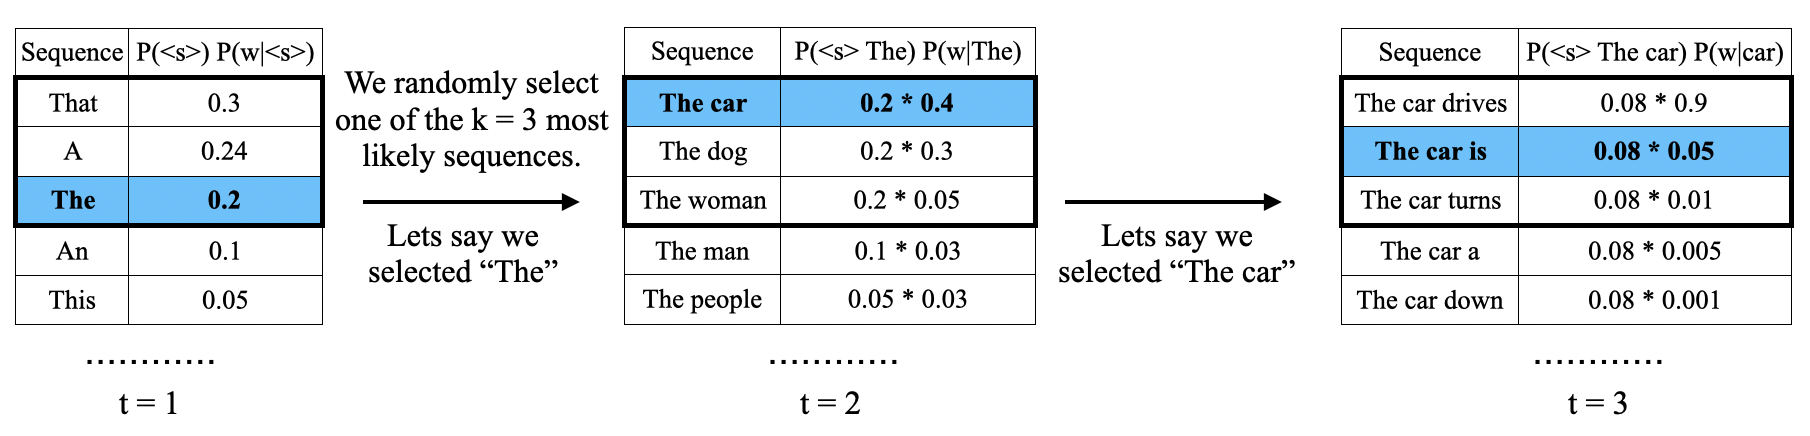
\includegraphics[width=0.92\textwidth]{images/top_k_sampling.png}
    \caption{Example of top-k random sampling. At each timestep t, the model generates the probability of the possible next word. Then, we randomly sample from the $k$ most likely candidates from this distribution. Here, we consider $k = 3$. \textbf{Bold} sequences represent the sampled candidate at each timestep.}
    \label{fig:top_k}
\end{figure}
    
    Once again, consider the bigram language model in Table \ref{tab:bigram_prob}.
    
    \begin{enumerate}
        \item (\textbf{1 pt}) Given the prefix string ``$\langle s\rangle\;I\;know$'', run the top-k sampling approach for the next 3 tokens.  Let $S$ be the set of output sequences that this approach could possibly generate at the end of 3 steps. What is the size of $S$? Assume $k = 2$ and $P(\langle s  \rangle\;I\;know) = 1$. You can just report the number.
        
        
        \item (\textbf{1 pt}) What is the sequence with maximum probability in $S$? Report the sequence and the probability of the sequence. 
        
        
        \item (\textbf{1 pt}) What is the sequence with  minimum probability in $S$? Report the sequence and the probability of the sequence.
        
        
    \end{enumerate}

    \item Let's say we are decoding a sentence of length $T$ using a language model with vocabulary size $V$. Report the time complexity in the big $O$ notation when the sentence is decoded using the following strategies:

    \begin{enumerate}
    \item (\textbf{1 pt}) Greedy search, where we store only the topmost sequence at each time step. 
    

    
    \item (\textbf{1 pt}) Beam search of width $k$, where we store the top-$k$ sequences at each time step: 


    
    \item (\textbf{1 pt}) Exhaustive search, where we store all the sequences at each time step: 
    
    
    \end{enumerate}

\end{enumerate}

\end{document}